\documentclass{standalone}
\usepackage{tikz}
\usetikzlibrary{patterns, positioning}


\begin{document}
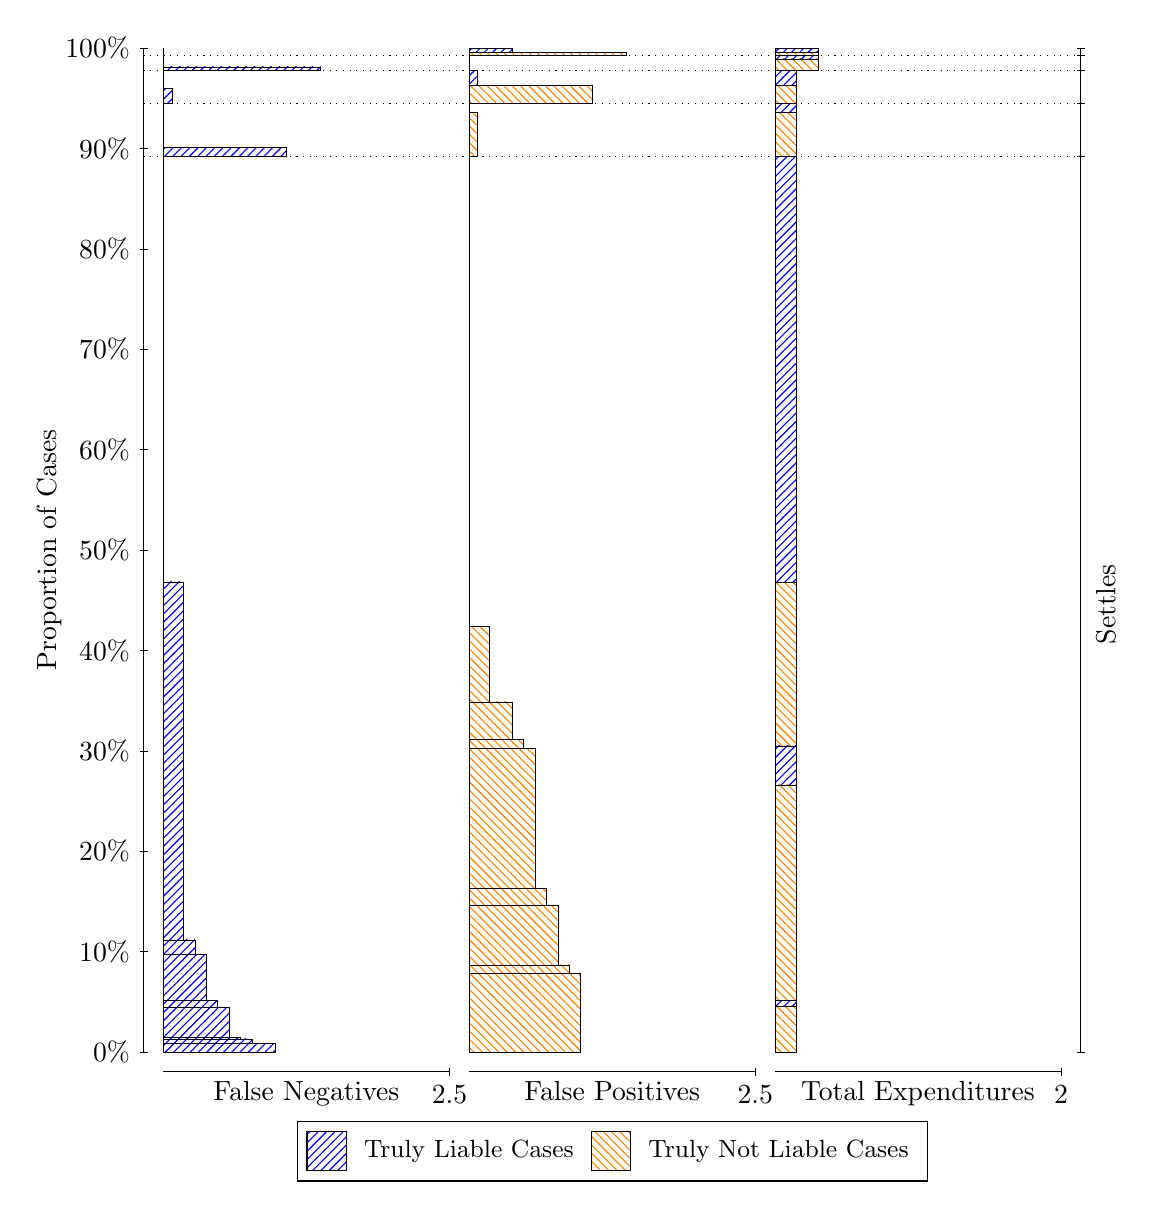
\begin{tikzpicture}
\draw[black, very thin] (1.5,1.75) -- (1.5,14.5);
\node[rotate=90, text=black, anchor=center] at (0.3, 8.125) {Proportion of Cases};
\draw[black, very thin] (1.45,1.75) -- (1.55,1.75);
\node[text=black, anchor=east] at (1.45, 1.75) {0\%};
\draw[black, very thin] (1.45,3.025) -- (1.55,3.025);
\node[text=black, anchor=east] at (1.45, 3.025) {10\%};
\draw[black, very thin] (1.45,4.3) -- (1.55,4.3);
\node[text=black, anchor=east] at (1.45, 4.3) {20\%};
\draw[black, very thin] (1.45,5.575) -- (1.55,5.575);
\node[text=black, anchor=east] at (1.45, 5.575) {30\%};
\draw[black, very thin] (1.45,6.85) -- (1.55,6.85);
\node[text=black, anchor=east] at (1.45, 6.85) {40\%};
\draw[black, very thin] (1.45,8.125) -- (1.55,8.125);
\node[text=black, anchor=east] at (1.45, 8.125) {50\%};
\draw[black, very thin] (1.45,9.4) -- (1.55,9.4);
\node[text=black, anchor=east] at (1.45, 9.4) {60\%};
\draw[black, very thin] (1.45,10.675) -- (1.55,10.675);
\node[text=black, anchor=east] at (1.45, 10.675) {70\%};
\draw[black, very thin] (1.45,11.95) -- (1.55,11.95);
\node[text=black, anchor=east] at (1.45, 11.95) {80\%};
\draw[black, very thin] (1.45,13.225) -- (1.55,13.225);
\node[text=black, anchor=east] at (1.45, 13.225) {90\%};
\draw[black, very thin] (1.45,14.5) -- (1.55,14.5);
\node[text=black, anchor=east] at (1.45, 14.5) {100\%};

\draw[black, very thin] (13.4,1.75) -- (13.4,14.5);
\draw[black, very thin] (13.35,1.75) -- (13.45,1.75);
\node[anchor=west] at (13.35, 1.75) {};
\draw[black, very thin] (13.35,13.123) -- (13.45,13.123);
\node[anchor=west] at (13.35, 13.123) {};
\draw[black, very thin] (13.35,13.798) -- (13.45,13.798);
\node[anchor=west] at (13.35, 13.798) {};
\draw[black, very thin] (13.35,14.219) -- (13.45,14.219);
\node[anchor=west] at (13.35, 14.219) {};
\draw[black, very thin] (13.35,14.405) -- (13.45,14.405);
\node[anchor=west] at (13.35, 14.405) {};
\draw[black, very thin] (13.35,14.5) -- (13.45,14.5);
\node[anchor=west] at (13.35, 14.5) {};

\draw[black, very thin, pattern color=blue, pattern=north east lines] (1.75,1.75) rectangle (3.167,1.8605);
\draw[black, very thin, pattern color=blue, pattern=north east lines] (1.75,1.8605) rectangle (2.8763,1.9149);
\draw[black, very thin, pattern color=blue, pattern=north east lines] (1.75,1.9149) rectangle (2.731,1.9315);
\draw[black, very thin, pattern color=blue, pattern=north east lines] (1.75,1.9315) rectangle (2.5857,2.3157);
\draw[black, very thin, pattern color=blue, pattern=north east lines] (1.75,2.3157) rectangle (2.4403,2.4071);
\draw[black, very thin, pattern color=blue, pattern=north east lines] (1.75,2.4071) rectangle (2.295,2.9907);
\draw[black, very thin, pattern color=blue, pattern=north east lines] (1.75,2.9907) rectangle (2.1497,3.1735);
\draw[black, very thin, pattern color=blue, pattern=north east lines] (1.75,3.1735) rectangle (2.0043,7.7214);
\draw[black, very thin, pattern color=orange, pattern=north west lines] (1.75,7.7214) rectangle (1.75,13.123);
\draw[black, very thin, pattern color=blue, pattern=north east lines] (1.75,13.123) rectangle (3.3123,13.239);
\draw[black, very thin, pattern color=orange, pattern=north west lines] (1.75,13.239) rectangle (1.75,13.798);
\draw[black, very thin, pattern color=blue, pattern=north east lines] (1.75,13.798) rectangle (1.859,13.99);
\draw[black, very thin, pattern color=orange, pattern=north west lines] (1.75,13.99) rectangle (1.75,14.219);
\draw[black, very thin, pattern color=blue, pattern=north east lines] (1.75,14.219) rectangle (3.7483,14.261);
\draw[black, very thin, pattern color=orange, pattern=north west lines] (1.75,14.261) rectangle (1.75,14.405);
\draw[black, very thin, pattern color=orange, pattern=north west lines] (1.75,14.405) rectangle (1.75,14.447);
\draw[black, very thin, pattern color=blue, pattern=north east lines] (1.75,14.447) rectangle (1.75,14.5);
\draw[black, very thin, pattern color=orange, pattern=north west lines] (5.6333,1.75) rectangle (7.0503,2.7445);
\draw[black, very thin, pattern color=orange, pattern=north west lines] (5.6333,2.7445) rectangle (6.905,2.8552);
\draw[black, very thin, pattern color=orange, pattern=north west lines] (5.6333,2.8552) rectangle (6.7597,3.608);
\draw[black, very thin, pattern color=orange, pattern=north west lines] (5.6333,3.608) rectangle (6.6143,3.8308);
\draw[black, very thin, pattern color=orange, pattern=north west lines] (5.6333,3.8308) rectangle (6.469,5.6102);
\draw[black, very thin, pattern color=orange, pattern=north west lines] (5.6333,5.6102) rectangle (6.3237,5.7179);
\draw[black, very thin, pattern color=orange, pattern=north west lines] (5.6333,5.7179) rectangle (6.1783,6.196);
\draw[black, very thin, pattern color=orange, pattern=north west lines] (5.6333,6.196) rectangle (5.8877,7.1519);
\draw[black, very thin, pattern color=blue, pattern=north east lines] (5.6333,7.1519) rectangle (5.6333,13.123);
\draw[black, very thin, pattern color=orange, pattern=north west lines] (5.6333,13.123) rectangle (5.7423,13.682);
\draw[black, very thin, pattern color=blue, pattern=north east lines] (5.6333,13.682) rectangle (5.6333,13.798);
\draw[black, very thin, pattern color=orange, pattern=north west lines] (5.6333,13.798) rectangle (7.1957,14.026);
\draw[black, very thin, pattern color=blue, pattern=north east lines] (5.6333,14.026) rectangle (5.7423,14.219);
\draw[black, very thin, pattern color=orange, pattern=north west lines] (5.6333,14.219) rectangle (5.6333,14.363);
\draw[black, very thin, pattern color=blue, pattern=north east lines] (5.6333,14.363) rectangle (5.6333,14.405);
\draw[black, very thin, pattern color=orange, pattern=north west lines] (5.6333,14.405) rectangle (7.6317,14.447);
\draw[black, very thin, pattern color=blue, pattern=north east lines] (5.6333,14.447) rectangle (6.1783,14.5);
\draw[black, very thin, pattern color=orange, pattern=north west lines] (9.5167,1.75) rectangle (9.7892,2.3358);
\draw[black, very thin, pattern color=blue, pattern=north east lines] (9.5167,2.3358) rectangle (9.7892,2.4069);
\draw[black, very thin, pattern color=orange, pattern=north west lines] (9.5167,2.4069) rectangle (9.7892,5.1421);
\draw[black, very thin, pattern color=blue, pattern=north east lines] (9.5167,5.1421) rectangle (9.7892,5.6367);
\draw[black, very thin, pattern color=orange, pattern=north west lines] (9.5167,5.6367) rectangle (9.7892,7.7176);
\draw[black, very thin, pattern color=blue, pattern=north east lines] (9.5167,7.7176) rectangle (9.7892,13.123);
\draw[black, very thin, pattern color=orange, pattern=north west lines] (9.5167,13.123) rectangle (9.7892,13.682);
\draw[black, very thin, pattern color=blue, pattern=north east lines] (9.5167,13.682) rectangle (9.7892,13.798);
\draw[black, very thin, pattern color=orange, pattern=north west lines] (9.5167,13.798) rectangle (9.7892,14.026);
\draw[black, very thin, pattern color=blue, pattern=north east lines] (9.5167,14.026) rectangle (9.7892,14.219);
\draw[black, very thin, pattern color=orange, pattern=north west lines] (9.5167,14.219) rectangle (10.062,14.363);
\draw[black, very thin, pattern color=blue, pattern=north east lines] (9.5167,14.363) rectangle (10.062,14.405);
\draw[black, very thin, pattern color=orange, pattern=north west lines] (9.5167,14.405) rectangle (10.062,14.447);
\draw[black, very thin, pattern color=blue, pattern=north east lines] (9.5167,14.447) rectangle (10.062,14.5);
\draw[black, dotted] (1.5,13.123) -- (13.4,13.123);
\draw[black, dotted] (1.5,13.798) -- (13.4,13.798);
\draw[black, dotted] (1.5,14.219) -- (13.4,14.219);
\draw[black, dotted] (1.5,14.405) -- (13.4,14.405);
\draw[black, very thin] (1.75,1.5) -- (5.3833,1.5);
\node[text=black, anchor=north] at (3.5667, 1.5) {False Negatives};
\draw[black, very thin] (5.3833,1.45) -- (5.3833,1.55);
\node[text=black, anchor=north] at (5.3833, 1.45) {2.5};

\draw[black, very thin] (5.6333,1.5) -- (9.2667,1.5);
\node[text=black, anchor=north] at (7.45, 1.5) {False Positives};
\draw[black, very thin] (9.2667,1.45) -- (9.2667,1.55);
\node[text=black, anchor=north] at (9.2667, 1.45) {2.5};

\draw[black, very thin] (9.5167,1.5) -- (13.15,1.5);
\node[text=black, anchor=north] at (11.333, 1.5) {Total Expenditures};
\draw[black, very thin] (13.15,1.45) -- (13.15,1.55);
\node[text=black, anchor=north] at (13.15, 1.45) {2};

\node[text=black, centered, rotate=90] at (13.72, 7.4366) {Settles};





\draw (7.449999999999999,1.5) node[draw=none] (baseCoordinate) {};
\begin{scope}[align=center]
        \matrix[scale=0.5, draw=black, below=0.5cm of baseCoordinate, nodes={draw}, column sep=0.1cm]{
            \node[rectangle, draw, minimum width=0.5cm, minimum height=0.5cm, pattern color=blue, pattern=north east lines] {}; &
            \node[draw=none, font=\small, text=black] (B) {Truly Liable Cases}; &
            \node[rectangle, draw, minimum width=0.5cm, minimum height=0.5cm, pattern color=orange, pattern=north west lines] {}; &
            \node[draw=none, font=\small, text=black] (B) {Truly Not Liable Cases}; \\
            };
\end{scope}

\end{tikzpicture}
\end{document}